
\begin{frame}
  \frametitle{Modelica: A Language for Modelling of Complex Physical Systems}
  % What is Modelica ?
  Modelica in few words
  \begin{itemize}
  \item A \textbf{language} and a \textbf{Standard Library}
  \item Object-Oriented and Equation based
  \item Multi-domains Modelling
  \item Non-proprietary
  \item Developed by the non-profit \textbf{Modelica Association}
  \item initiated in September 1996 by Hilding Elmqvist
  \item First version on Sept. 1997  $\rightarrow$ 3.4 on April 2017
  \item Commercial front-ends: e.g.\@ Dymola
  \item Open Source front-ends: \textbf{OpenModelica} and \textbf{JModelica} \\[1em]
  \end{itemize}
  % \begin{columns}
  %   \begin{column}[t]{.65\textwidth}
  % \end{column}
  % \begin{column}[t]{.35\textwidth}
  %   Front-Ends
  %   \begin{itemize}
  %   \item Commercial : e.g.\@ Dymola
  %   \item Open Source : \\
  %     \begin{itemize}
  %     \item OpenModelica
  %     \item JModelica
  %     \end{itemize}
  %   \end{itemize}
  % \end{column}
  % \end{columns}
  {\tiny%
    \begin{tabbing}
      To go further \=%
      \url{https://www.modelica.org} \\
      \> \href{https://www.openmodelica.org/images/docs/tutorials/modelicatutorialfritzson.pdf}{
        Introduction to Object-Oriented Modeling and Simulation with OpenModelica - Peter Fritzson}
      \end{tabbing}%
    }
  \begin{textblock}{6}(13,7)
    
\includegraphics[width=2cm]{images/modelica-logo.jpg}
  \end{textblock}
\end{frame}

\begin{frame}[fragile]
  \frametitle{Modelica: Bouncing-ball Example}
  \begin{columns}[T]
    \begin{column}{.6\textwidth}
      \fontsize{8pt}{8pt}\selectfont
\begin{Verbatim}[commandchars=\\\{\}]
\colorG{model} BouncingBall
  \colorG{parameter} Real e=0.7 \colorR{"coefficient of restitution"};
  \colorG{parameter} Real g=9.81 \colorR{"gravity acceleration"};
  Real h(start=1) \colorR{"height of ball"};
  Real v \colorR{"velocity of ball"};
  Boolean flying(start=true) \colorR{"true, if ball is flying"};
  Boolean impact;
  Real v_new;

\colorM{equation}
  impact = h <= 0;
  \colorB{der}(v) = \colorM{if} flying \colorM{then} -g \colorM{else} 0;
  \colorB{der}(h) = v;

  \colorO{// Triggered when one of theses conditions are true}
  \colorM{when} \{h <= 0 \colorM{and} v <= 0, impact\} \colorM{then}
    v_new = \colorM{if} \colorB{edge}(impact) \colorM{then} -e*\colorB{pre}(v) \colorM{else} 0;
    flying = v_new > 0;
    \colorB{reinit}(v, v_new);
  \colorM{end when};

\colorG{end} BouncingBall;
\end{Verbatim}
      \normalsize
    \end{column}
    \begin{column}{.4\textwidth}
      \small
      Netwton's Law
      \begin{align*}
        \frac{dh}{dt} &= v \\
        \frac{dv}{dt} &= \frac{d^2 h}{dt^2} = -g
      \end{align*}
      At impact, lost some energy
      $$ v^\prime = -e v $$
      and go upwards
      \newcommand*{\ClipSep}{1mm}%
      \begin{tikzpicture}
        \begin{scope}
          \clip [rounded corners=2mm] (0,0) rectangle coordinate (centerpoint) ++(2cm,3cm);
          \node [inner sep=0pt] at (centerpoint) {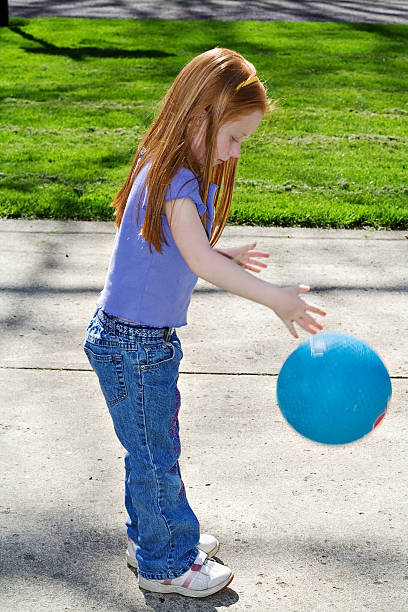
\includegraphics[width=2cm]{images/bouncing-ball-girl.jpg}};
          % \node [inner sep=0pt] at (0, 0) {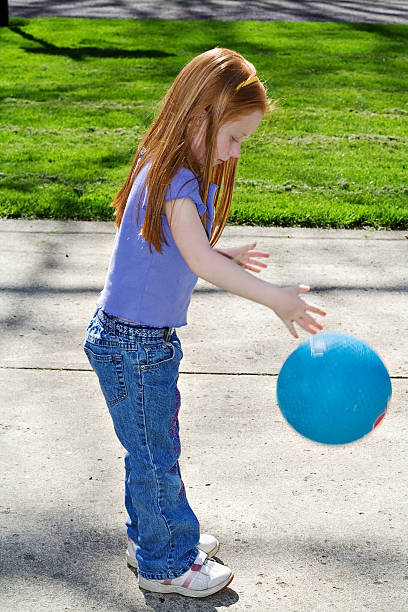
\includegraphics[width=2cm]{images/bouncing-ball-girl.jpg}};
          % \draw [white, rounded corners=\ClipSep, line width=\ClipSep]
          % (current bounding box.north west) --
          % (current bounding box.north east) --
          % (current bounding box.south east) --
          % (current bounding box.south west) -- cycle;
        \end{scope}
      \end{tikzpicture}
      \normalsize
    \end{column}
  \end{columns}
\end{frame}

\begin{frame}[fragile]
  \frametitle{Modelica: Circuit with Annotations (Schema)}
  \fontsize{5pt}{5pt}\selectfont
\begin{Verbatim}[commandchars=\\\{\}]
\colorG{model} SimpleRectifierWithTransformer
  \colorY{Modelica.Electrical.Analog.Sources.SineVoltage} ac_line(V = 230, freqHz = 50);
  \colorY{Modelica.Electrical.Analog.Basic.Capacitor} capacitor(C = 0.00005);
  \colorY{Modelica.Electrical.Analog.Basic.Ground} ground;
  \colorY{Modelica.Electrical.Analog.Ideal.IdealDiode} diode(Vknee = 0.5);
  \colorY{Modelica.Electrical.Analog.Basic.Resistor} load_resistor(R = 1000.0);
  \colorY{Modelica.Electrical.Analog.Ideal.IdealTransformer} transformer(n = 10, Lm1 = 1);
  \colorY{Modelica.Electrical.Analog.Sources.SineVoltage} sinevoltage1
    \colorB{annotation}(\colorO{Placement(visible = true, transformation(origin = {-78.7769,-10.3538}, extent = {{-10,-10},{10,10}}, rotation = -90))});
  \colorY{Modelica.Electrical.Analog.Basic.Transformer} transformer1 \colorB{annotation}(\ldots);
  \colorY{Modelica.Electrical.Analog.Semiconductors.Diode} diode1 \colorB{annotation}(\ldots);
  \colorY{Modelica.Electrical.Analog.Basic.Resistor} resistor1 \colorB{annotation}(\ldots);
  \colorY{Modelica.Electrical.Analog.Basic.Capacitor} capacitor1 \colorB{annotation}(\ldots);
  \colorY{Modelica.Electrical.Analog.Basic.Ground} ground1 \colorB{annotation}(\ldots);
\colorM{equation}
  \colorB{connect}(resistor1.n, ground1.p)
    \colorB{annotation}(\colorO{Line(points = {{22.286, -18.6196}, {22.286, -25.0637}, {22.5062, -25.0637}, {22.5062, -25.0637}})});
  \colorB{connect}(capacitor1.n, transformer1.n2) \colorB{annotation}(\ldots);
  \colorB{connect}(resistor1.n, capacitor1.n) \colorB{annotation}(\ldots);
  \colorB{connect}(capacitor1.p, resistor1.p) \colorB{annotation}(\ldots);
  \colorB{connect}(diode1.n, capacitor1.p) \colorB{annotation}(\ldots);
  \colorB{connect}(transformer1.p2, diode1.p) \colorB{annotation}(\ldots);
  \colorB{connect}(sinevoltage1.n, transformer1.n1) \colorB{annotation}(\ldots);
  \colorB{connect}(sinevoltage1.p, transformer1.p1) \colorB{annotation}(\ldots);
  \colorB{connect}(ac_line.p, transformer.p1);
  \colorB{connect}(ac_line.n, transformer.n1);
  \colorB{connect}(ac_line.n, ground.p);
  \colorB{connect}(transformer.p2, diode.p);
  \colorB{connect}(transformer.n2, ground.p);
  \colorB{connect}(diode.n, capacitor.p);
  \colorB{connect}(diode.n, load_resistor.p);
  \colorB{connect}(capacitor.n, ground.p);
  \colorB{connect}(load_resistor.n, ground.p);
  \colorB{annotation}(\colorO{Diagram(coordinateSystem(extent = {{-100, -100}, {100, 100}}, preserveAspectRatio = true, initialScale = 0.1, grid = {2, 2}))});
\colorG{end} SimpleRectifierWithTransformer;
\end{Verbatim}
  \normalsize
  % \begin{center}
  % \end{center}
  \begin{flushright}
   \tiny%
    To go further \href{https://www.modelica.org/events/modelica2009/Proceedings/memorystick/pages/papers/0019/0019.pdf}{SPICE3 Modelica Library}
  \end{flushright}
  \begin{textblock}{8}(7,4.5)
    \begin{enumerate}
    \item Define devices
    \item \texttt{\colorB{connect}(resistor1.n, ground1.p)} \\[1em]
    \end{enumerate}
    \attention{} \alert{Modelica performs Transient Analysis}
  \end{textblock}
\end{frame}

\begin{frame}
  \frametitle{Modelica: Open Source Front-Ends}
  \begin{enumerate}
  \item \textbf{OpenModelica} \hfill {\small \url{https://www.openmodelica.org}}
    \begin{itemize}
    \item Supported by a non-profit organization : Open Source Modelica Consortium (OSMC)
    \item OSMC Public License $\approx$ GPL V3
    \item \textbf{Provide an IDE} : OMEdit
    \item \textbf{Based on \Cpp{} and Corba}
    \item V1.12 released on May 2017
    \item \href{https://build.openmodelica.org}{Packages} available on some Linux Distributions \\[1em]
    \end{itemize}
  \item \textbf{JModelica} \hfill {\small \url{http://jmodelica.org}}
    \begin{itemize}
    \item Started at Department of Automatic Control, Lund University
    \item Supported by Modelon AB
    \item GPL V3
    \item \textbf{Based on Java and Python}
    \item V2.0 released on May 2017
    \end{itemize}
  \end{enumerate}
  \centerline{\attention{} \alert{Packages are welcome since compilation can be tricky \ldots}}
\end{frame}

\begin{frame}
  \frametitle{OMEdit Screenshots}
  \begin{columns}
    \begin{column}[c]{.5\textwidth}
      \begin{center}
        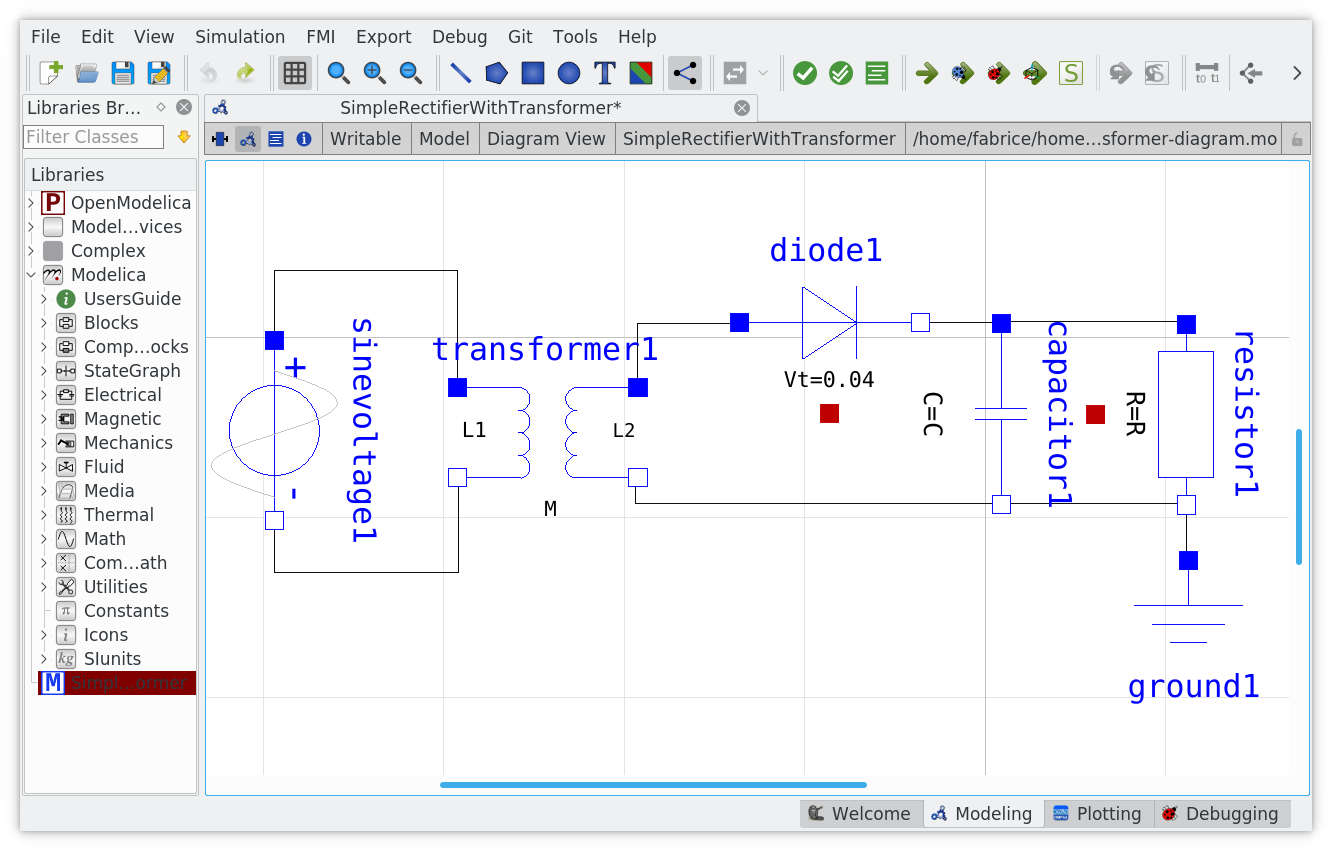
\includegraphics[width=1.\textwidth]{images/omedit-schema.png}
      \end{center}
    \end{column}
    \begin{column}[c]{.5\textwidth}
      \begin{center}
        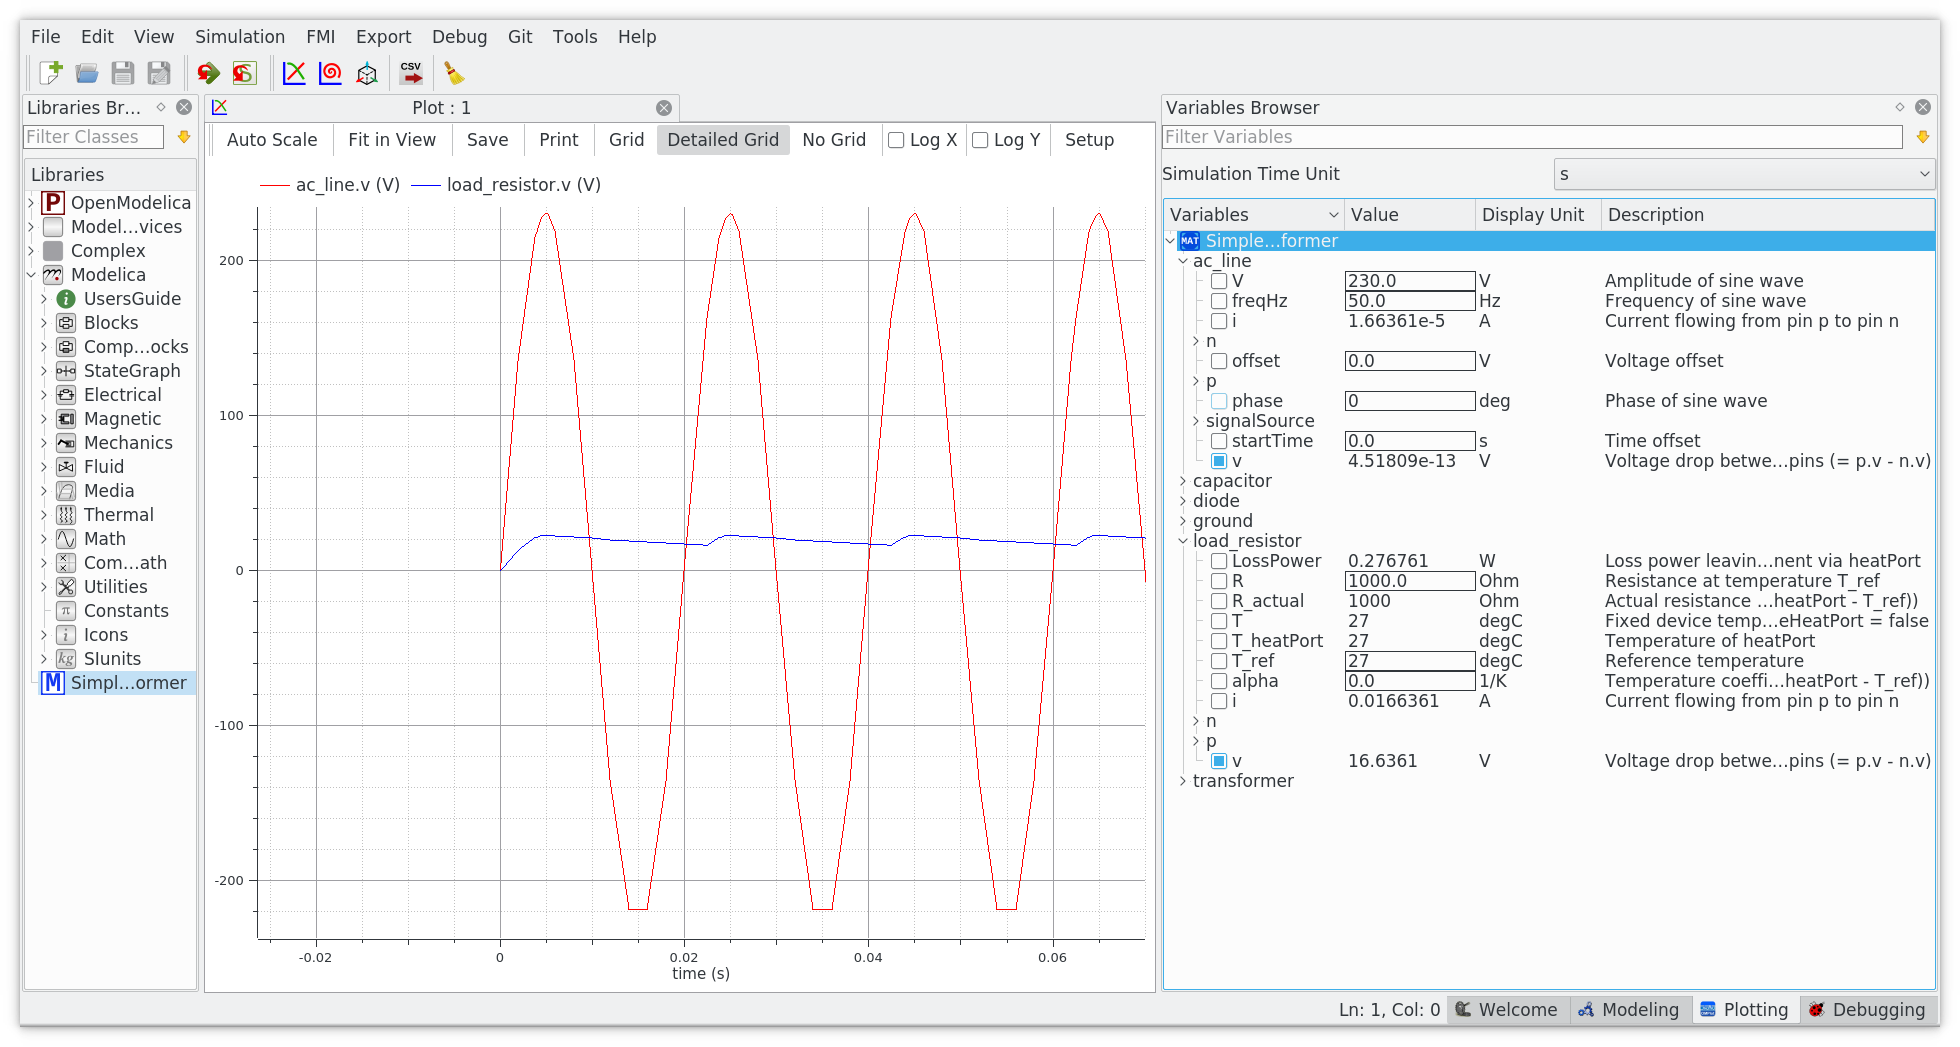
\includegraphics[width=1.\textwidth]{images/omedit-plot.png}
      \end{center}
    \end{column}
  \end{columns}
\end{frame}

\begin{frame}[fragile]
  \frametitle{Using OpenModelica with Python}
  \begin{columns}[T]
    \begin{column}{.5\textwidth}
      \fontsize{9pt}{9pt}\selectfont
\begin{Verbatim}[commandchars=\\\{\}]
\colorB{from} OMPython \colorB{import} ModelicaSystem

mod = ModelicaSystem(\colorO{'bouncing-ball.mo'},
                     \colorO{'BouncingBall'})

mod.setSimulationOptions(stopTime=3)
mod.simulate()

mod.getSolutions()
t = mod.getSolutions(\colorO{'time'})
h = mod.getSolutions(\colorO{'h'})

\colorB{import} pylab
pylab.grid()
pylab.plot(t, h)
pylab.xlabel(\colorO{'time [s]'})
pylab.ylabel(\colorO{'[height]'})
\end{Verbatim}
      \normalsize
    \end{column}
    \begin{column}{.5\textwidth}
      \begin{center}
        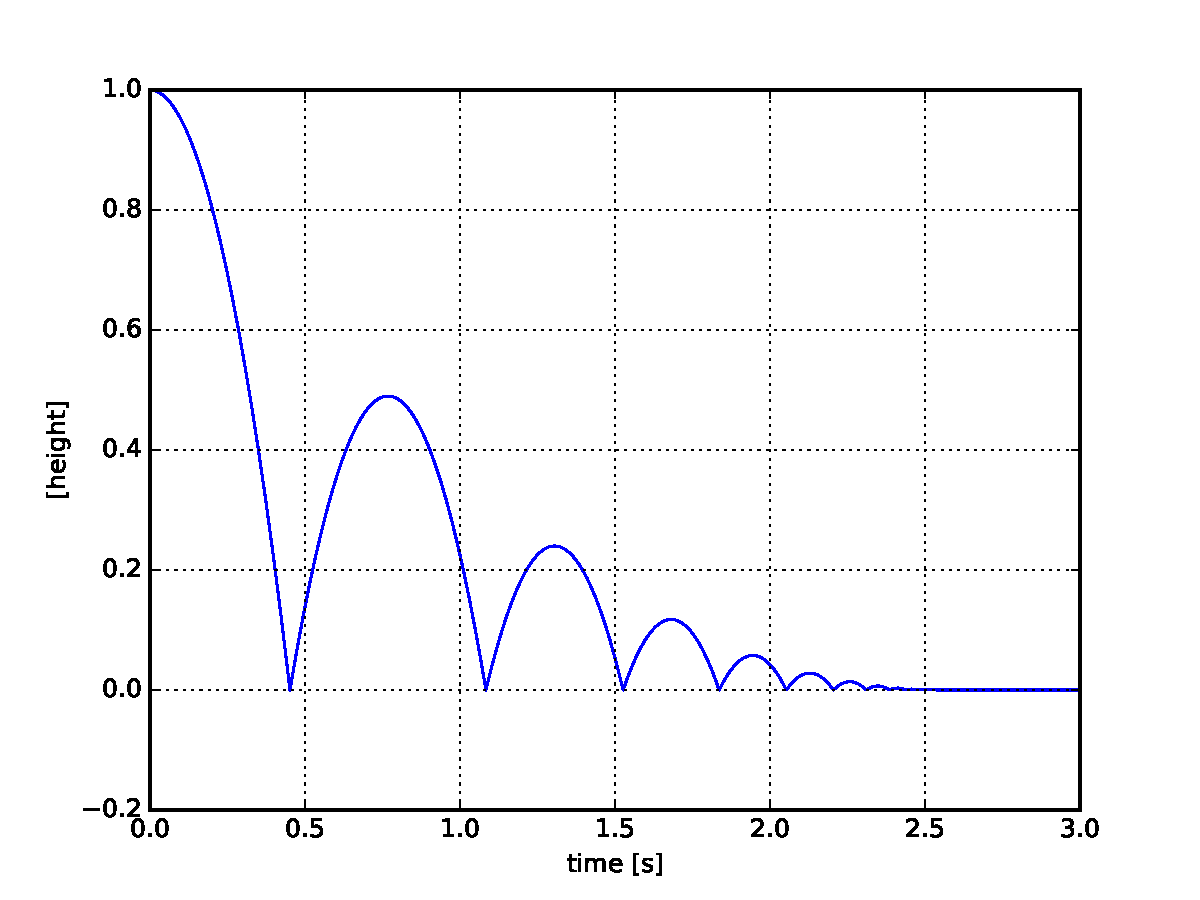
\includegraphics[width=1.\textwidth]{figures/bouncing-ball-height.pdf}
      \end{center}
    \end{column}
  \end{columns}
  \vspace{.5em}
  \centerline{\textbf{Model is compiled to C}}
  \begin{flushright}
    \tiny%
    To go further
    \href{https://www.openmodelica.org/doc/OpenModelicaUsersGuide/latest/ompython.html}{OpenModelica Python Interface}
    % https://www.fabrice-salvaire.fr/en/blog/first-steps-with-openmodelica/
  \end{flushright}
\end{frame}

%%% Local Variables:
%%% mode: latex
%%% TeX-master: "master"
%%% End:
